\documentclass[11pt,a4paper]{article}

\usepackage[margin=1.9cm]{geometry}
\usepackage[T1]{fontenc}
\usepackage[utf8]{inputenc}
\usepackage{lmodern}
\usepackage{amsmath,amssymb,booktabs,enumitem,microtype,hyperref,xcolor,tcolorbox,tabularx,parskip,tikz}
\usepackage{titlesec}
\usetikzlibrary{arrows.meta,positioning,fit,calc,shapes.geometric}

\hypersetup{colorlinks=true,linkcolor=black!75,urlcolor=blue!45!black,citecolor=black!75}
\tcbuselibrary{skins,breakable}

\titleformat{\section}{\large\bfseries\color{blue!40!black}}{\thesection}{0.5em}{}
\titleformat{\subsection}{\bfseries\color{blue!28!black}}{\thesubsection}{0.4em}{}
\setlist[itemize]{leftmargin=1.15em,itemsep=0.18em,topsep=0.2em}
\setlist[enumerate]{leftmargin=1.25em,itemsep=0.18em,topsep=0.2em}

\newtcolorbox{keybox}[1][]{
  colback=blue!4!white,colframe=blue!45!black,fonttitle=\bfseries,
  title={#1},breakable,left=5pt,right=5pt,top=3pt,bottom=3pt,boxrule=0.55pt
}
\newtcolorbox{linkbox}[1][]{
  colback=teal!4!white,colframe=teal!50!black,fonttitle=\bfseries,
  title={#1},breakable,left=5pt,right=5pt,top=3pt,bottom=3pt,boxrule=0.55pt
}
\newtcolorbox{warnbox}[1][]{
  colback=orange!6!white,colframe=orange!55!black,fonttitle=\bfseries,
  title={#1},breakable,left=5pt,right=5pt,top=3pt,bottom=3pt,boxrule=0.55pt
}
\newtcolorbox{formulabox}{
  colback=black!2!white,colframe=black!30,left=5pt,right=5pt,top=4pt,bottom=4pt,boxrule=0.45pt
}

\newcommand{\R}{\mathbb{R}}
\newcommand{\eps}{\varepsilon}
\newcommand{\norm}[1]{\|#1\|}

\title{%
  \textbf{AML --- White-Box Konzeptübersicht}\\[0.25em]
  {\large Vorlesung \emph{Adversarial Machine Learning} (Rieck) + Papers}
}
\author{Extrem kompakte Landkarte: Begriffe, Formeln, Verbindungen}
\date{}

\begin{document}
\maketitle
\vspace{-1.4em}

\begin{keybox}[Ziel dieses Dokuments]
Alles Wichtige aus den Slides \texttt{aml-advwhite-small} an einem Ort ---
\textbf{was} die Konzepte sind und \textbf{wie} sie zusammenhängen.
Papers (Goodfellow, Carlini\&Wagner) nur als Brücke, wo sie die Slides vertiefen.
\end{keybox}

%======================================================================
\section{Landkarte: Wie hängt alles zusammen?}

\begin{center}
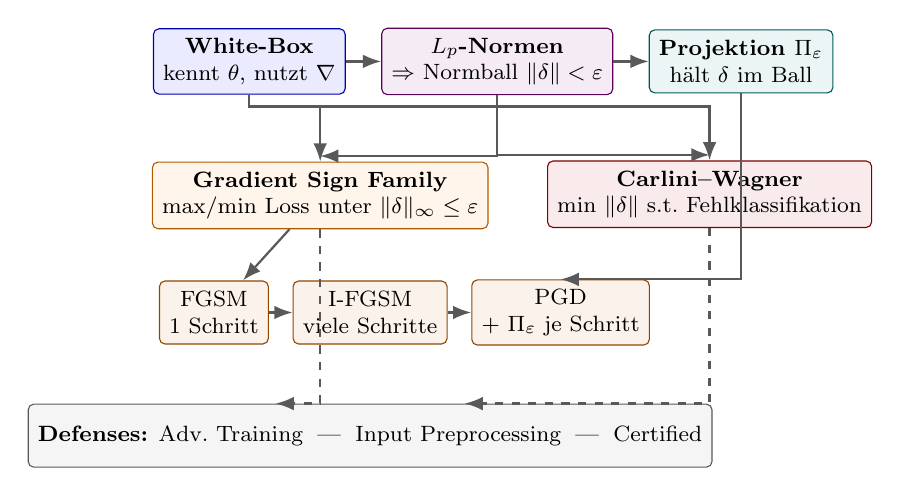
\begin{tikzpicture}[
  font=\footnotesize,
  box/.style={draw=#1!70!black, fill=#1!8, rounded corners=2pt,
              align=center, inner sep=3.5pt, minimum height=0.8cm},
  arr/.style={-{Latex}, thick, gray!70!black}
]
  % Zeile 1: Grundlagen
  \node[box=blue] (wb) {\textbf{White-Box}\\kennt $\theta$, nutzt $\nabla$};
  \node[box=violet, right=0.45cm of wb] (norm) {\textbf{$L_p$-Normen}\\$\Rightarrow$ Normball $\|\delta\|<\eps$};
  \node[box=teal, right=0.45cm of norm] (proj) {\textbf{Projektion $\Pi_\eps$}\\hält $\delta$ im Ball};

  % Zeile 2: zwei Angriffsphilosophien
  \node[box=orange, below=0.85cm of wb, xshift=0.9cm] (gsm)
    {\textbf{Gradient Sign Family}\\max/min Loss unter $\|\delta\|_\infty\le\eps$};
  \node[box=red!70!black, below=0.85cm of proj, xshift=-0.4cm] (cw)
    {\textbf{Carlini--Wagner}\\min $\|\delta\|$ s.t.\ Fehlklassifikation};

  % Zeile 3: GSM-Kette
  \node[box=orange!80!black, below=0.65cm of gsm, xshift=-1.35cm] (fgsm) {FGSM\\1 Schritt};
  \node[box=orange!80!black, right=0.3cm of fgsm] (ifgsm) {I-FGSM\\viele Schritte};
  \node[box=orange!80!black, right=0.3cm of ifgsm] (pgd) {PGD\\+ $\Pi_\eps$ je Schritt};

  % Zeile 4: Defenses
  \node[box=gray, below=0.75cm of ifgsm] (def)
    {\textbf{Defenses:} Adv.\ Training \;|\; Input Preprocessing \;|\; Certified};

  \draw[arr] (wb) -- (norm);
  \draw[arr] (norm) -- (proj);
  \draw[arr] (wb.south) -- ++(0,-0.15) -| (gsm.north);
  \draw[arr] (wb.south) -- ++(0,-0.15) -| (cw.north);
  \draw[arr] (norm.south) |- ([yshift=2pt]gsm.north);
  \draw[arr] (norm.south) |- ([yshift=2pt]cw.north);
  \draw[arr] (proj.south) |- (pgd.north);
  \draw[arr] (gsm) -- (fgsm);
  \draw[arr] (fgsm) -- (ifgsm);
  \draw[arr] (ifgsm) -- (pgd);
  \draw[arr, dashed] (gsm.south) |- ([xshift=-1.2cm]def.north);
  \draw[arr, dashed] (cw.south) |- ([xshift=1.2cm]def.north);
\end{tikzpicture}
\end{center}

\begin{linkbox}[Eine Zeile Zusammenfassung]
\textbf{Normen} sagen, was ``klein'' heißt.\quad
\textbf{GSM/PGD} schieben entlang des Loss-Gradienten im $\eps$-Ball.\quad
\textbf{C\&W} sucht die \emph{kleinste} Störung, die die Klasse kippt.
\end{linkbox}

%======================================================================
\section{Notation (einmal, dann überall gleich)}

\begin{center}
\renewcommand{\arraystretch}{1.2}
\begin{tabularx}{\textwidth}{@{}>{\bfseries}l X@{}}
\toprule
Symbol & Bedeutung \\
\midrule
$x\in\R^d$ & Original-Eingabe (z.\,B.\ Bild in $[0,1]^d$) \\
$y$ & wahres Label (Ground Truth) \\
$t\neq y$ & Zielklasse (nur bei targeted) \\
$f$ / $\theta$ & Modell / Parameter (White-Box: beides bekannt) \\
$z(x)$ & \textbf{Logits} (Ausgabe \emph{vor} Softmax) \\
$\delta$ & Störung; $\bar x = x+\delta$ = adversariales Beispiel \\
$\eps$ & Budget: erlaubt ist nur $\|\delta\| < \eps$ (Normball) \\
$\ell$ & Loss (z.\,B.\ Cross-Entropy) \\
\bottomrule
\end{tabularx}
\end{center}

%======================================================================
\section{Teil 1 --- Vektornormen, Normball, Projektion}

\subsection{Vier Normen --- was sie messen}
Norm $\|\cdot\|$ misst die ``Größe'' der Störung $\delta$. In AML proxy für
\emph{menschliche Unauffälligkeit}.

\begin{center}
\renewcommand{\arraystretch}{1.25}
\begin{tabular}{@{}llp{5.8cm}@{}}
\toprule
\textbf{Norm} & \textbf{Formel} & \textbf{Intuition für Angriffe} \\
\midrule
$L_0$ & Anzahl Nicht-Nullen & wenige Pixel stark ändern \\
$L_1$ & $\sum_i |\delta_i|$ & Manhattan / Summe der Beträge \\
$L_2$ & $\sqrt{\sum_i \delta_i^2}$ & viele Pixel etwas (``Energie'') \\
$L_\infty$ & $\max_i |\delta_i|$ & kein Pixel mehr als $\eps$ \\
\bottomrule
\end{tabular}
\end{center}

\textbf{Beispiel} $x=(0,3,4)$: $\|x\|_0=2$, $\|x\|_1=7$, $\|x\|_2=5$, $\|x\|_\infty=4$.

\subsection{Normball}
\[
\{\bar x : \|\bar x - x\| < \eps\}
\quad=\quad
\{x+\delta : \|\delta\| < \eps\}
\]
Alles Erlaubte liegt \emph{innerhalb} dieses Balls um $x$.

\subsection{Projektion $\Pi_\eps$}
Mappt einen Vektor zurück \emph{auf/in} den Normball:
\[
\Pi_\eps(v)
=
\begin{cases}
v & \text{falls }\|v\|_p < \eps,\\
s(v) & \text{sonst.}
\end{cases}
\]
\begin{itemize}
  \item $L_2$: Skalierung $s(v)=v\cdot\eps/\|v\|_2$
  \item $L_\infty$: Clamping $s(v)=\min(\max(v,-\eps),\eps)$
\end{itemize}

\begin{linkbox}[Verbindung zu Angriffen]
FGSM nutzt die Form des $L_\infty$-Balls direkt ($\delta=\eps\cdot\operatorname{sign}(g)$).\\
PGD braucht $\Pi_\eps$ nach jedem Schritt.\\
C\&W \emph{minimiert} die Norm statt ein festes $\eps$ vorzugeben.
\end{linkbox}

%======================================================================
\section{Teil 2 --- Was ist ein White-Box Adversarial Example?}

\begin{formulabox}
\textbf{Ziel (Integrity):} Vorhersage $f$ bei Inferenz täuschen.\\[0.3em]
Finde kleines $\delta$ mit
\[
f(x+\delta)\neq y
\qquad\text{und}\qquad
\|\delta\|<\eps.
\]
\end{formulabox}

\textbf{White-Box} $=$ Angreifer kennt Architektur und Parameter $\theta$ und
darf Gradienten $\nabla_x$ / $\nabla_\delta$ berechnen.

\begin{warnbox}[Problem-Space vs.\ Feature-Space]
Feature-Space: Störung direkt auf dem Modellinput (Pixel, Embeddings).\\
Problem-Space: Störung muss in der realen Welt gültig bleiben
(Foto, Audio, \ldots). Die Vorlesung startet im Feature-Space.
\end{warnbox}

%======================================================================
\section{Teil 3 --- Gradient Sign Methods}

Idee: Die Störung folgt dem \textbf{Gradienten des Loss} --- der Richtung,
in der die Vorhersage am schnellsten schlechter (oder zur Zielklasse besser) wird.

\subsection{Zwei Angriffsziele}
\begin{center}
\renewcommand{\arraystretch}{1.3}
\begin{tabularx}{\textwidth}{@{}>{\bfseries}p{2.4cm} X@{}}
\toprule
Untargeted &
$\displaystyle\arg\max_\delta\,\ell\big(f(x+\delta),\,y\big)$
\quad s.t.\ $\|\delta\|<\eps$
\hfill (Loss der \emph{wahren} Klasse hoch) \\
\midrule
Targeted &
$\displaystyle\arg\min_\delta\,\ell\big(f(x+\delta),\,t\big)$
\quad s.t.\ $\|\delta\|<\eps$, $t\neq y$
\hfill (Loss der \emph{Zielklasse} runter) \\
\bottomrule
\end{tabularx}
\end{center}

\subsection{FGSM --- ein Schritt}
Gradient $g=\nabla_\delta\,\ell(f(x+\delta),y)$.
Skaliertes $g$ rutscht leicht aus dem Ball; bei großem $\alpha$ clampen alle
Koordinaten auf $\pm\eps$. Deshalb der Sign-Trick:

\begin{formulabox}
\[
\boxed{\delta \;=\; \eps\cdot\operatorname{sign}(g)}
\qquad\text{(klassisch: }
\bar x = x + \eps\cdot\operatorname{sign}(\nabla_x J(\theta,x,y))
\text{)}
\]
\end{formulabox}
$\Rightarrow$ natürlich an $L_\infty$ gekoppelt, extrem schnell, oft schwach.

\subsection{I-FGSM --- viele kleine Schritte}
\begin{formulabox}
\[
\delta_k \;=\; \delta_{k-1} + \alpha\cdot\operatorname{sign}(g_{k-1})
\]
\end{formulabox}
Neue Hyperparameter: Schrittweite $\alpha$, Iterationen $k$.
Früh abbrechen, sobald die Entscheidungsgrenze überschritten ist.
\textbf{Problem:} $\delta$ kann den Normball verlassen.

\subsection{PGD --- I-FGSM + Projektion}
\begin{formulabox}
\[
\boxed{\delta_k \;=\; \Pi_\eps\big(\delta_{k-1} + \alpha\cdot\operatorname{sign}(g_{k-1})\big)}
\]
\end{formulabox}

\begin{linkbox}[Kette merken]
$\textbf{FGSM}$ $=$ 1× Gradient-Sign\quad$\to$\quad
$\textbf{I-FGSM}$ $=$ FGSM iteriert\quad$\to$\quad
$\textbf{PGD}$ $=$ I-FGSM + $\Pi_\eps$ nach jedem Schritt.\\
PGD gilt als Standard-\textbf{starke} $L_\infty$-Baseline zur Defense-Evaluation.
\end{linkbox}

%======================================================================
\section{Teil 4 --- Carlini--Wagner (andere Philosophie)}

\subsection{Ausgangsproblem}
Statt Loss zu maximieren: \textbf{Norm minimieren}, Klasse erzwingen:
\begin{formulabox}
\[
\arg\min_\delta\ \|\delta\|
\quad\text{s.t.}\quad
f(x+\delta)=t,\quad x+\delta\in[0,1]^d.
\]
\end{formulabox}
Zwei harte Punkte: (1)~diskrete Klassenbedingung, (2)~Box $[0,1]^d$.

\subsection{Trick 1 --- weiche Nebenbedingung $A$}
Ersetze $f(\bar x)=t$ durch $A(\bar x)\le 0 \;\Leftrightarrow\;$ Angriff erfolgreich:
\[
\arg\min_\delta\ \|\delta\| + c\cdot A(\bar x)
\quad\text{s.t.}\quad
\bar x\in[0,1]^d.
\]
$c>0$ steuert Tradeoff Distanz vs.\ Erfolg (oft Binary Search).

Empirisch starke Wahl auf \textbf{Logits} $z$ (nicht Softmax):
\begin{formulabox}
\[
A(\bar x)
=
\max\Big(0,\;
\max_{i\neq t} z(\bar x)_i - z(\bar x)_t
\Big)
\]
\end{formulabox}
$z_t$ soll größer sein als alle anderen Logits. Softmax-Objectives können
numerisch ``sterben'' (Gradient $\approx 0$).

\subsection{Trick 2 --- Box weg via $\tanh$}
\[
\delta \;=\; \tfrac12\big(\tanh(w)+1\big) - x
\quad\Rightarrow\quad
\bar x=\tfrac12(\tanh(w)+1)\in(0,1)^d.
\]
Optimierung ist dann \textbf{unbeschränkt} über $w$ (z.\,B.\ Adam).

\subsection{C\&W-$L_2$ (Kernformel der Vorlesung)}
\begin{formulabox}
\[
\arg\min_w\;
\Big\|
\tfrac12(\tanh(w)+1)-x
\Big\|_2^{\!2}
\;+\;
c\cdot A\!\Big(\tfrac12(\tanh(w)+1)\Big)
\]
\end{formulabox}
$L_0$/$L_\infty$-Varianten: andere äußere Schleifen (Pixel fixieren bzw.\ $\tau$-Schwellwert);
Innen oft wieder $L_2$-artige Optimierung --- Details im Paper.

\begin{linkbox}[GSM vs.\ C\&W]
\textbf{GSM/PGD:} festes Budget $\eps$, Loss pushen.\\
\textbf{C\&W:} kleinstmögliche Distanz suchen, Erfolg über $A\le 0$ erzwingen.\\
Beide sind White-Box und gradientenbasiert --- unterschiedliche Zielfunktion.
\end{linkbox}

%======================================================================
\section{Vergleichstabelle aller Angriffe}

\begin{center}
\renewcommand{\arraystretch}{1.22}
\footnotesize
\begin{tabular}{@{}lcccc@{}}
\toprule
& \textbf{FGSM} & \textbf{I-FGSM} & \textbf{PGD} & \textbf{C\&W} \\
\midrule
Idee & 1 Sign-Schritt & viele Schritte & + Projektion & min Norm + $A$ \\
Typ.\ Norm & $L_\infty$ & $L_\infty$ & $L_\infty$ & $L_0,L_2,L_\infty$ \\
Budget & fest $\eps$ & fest $\eps$ & fest $\eps$ & sucht kleines $\|\delta\|$ \\
Geschwindigkeit & sehr schnell & mittel & mittel & langsam \\
Stärke & schwach & stärker & stark & sehr stark \\
Braucht $\Pi_\eps$? & implizit & oft ja & \textbf{ja} & nein ($\tanh$) \\
\bottomrule
\end{tabular}
\end{center}

\vspace{0.35em}
Historische Brücke (Papers, nicht Schwerpunkt der Slides):
\textbf{L-BFGS} (Szegedy) = frühe Optimierung $\min c\|x'-x\|_2^2+\mathrm{loss}$ ---
stark aber teuer; motivierte FGSM (schnell) und später C\&W (besseres $f$/Logits).

%======================================================================
\section{Defenses (nur Überblick aus den Slides)}

Keine allgemein starke Defense --- aktives Forschungsfeld:
\begin{enumerate}
  \item \textbf{Adversarial Training:} mit Adv.\ Examples nachtrainieren
        (oft FGSM/PGD on-the-fly). Robustheit gilt nur gegen die genutzte Attack-Stärke.
  \item \textbf{Input Preprocessing:} Transformationen, die Störungen abschwächen.
  \item \textbf{Certified Defenses:} Garantien innerhalb eines Normballs.
\end{enumerate}

\begin{warnbox}[Evaluation-Regel]
Eine Defense nur gegen FGSM testen reicht nicht.
Starke Angriffe (PGD, C\&W) sind der Maßstab --- Kernbotschaft von Carlini\&Wagner.
\end{warnbox}

%======================================================================
\section{Begriffs-Netz (Schnelllookup)}

\begin{center}
\renewcommand{\arraystretch}{1.18}
\begin{tabularx}{\textwidth}{@{}>{\bfseries}p{3.1cm} X@{}}
\toprule
Begriff & Hängt zusammen mit \ldots \\
\midrule
White-Box & $\theta$ bekannt $\Rightarrow$ Gradienten $\Rightarrow$ GSM \& C\&W möglich \\
$L_p$-Norm & definiert ``klein''; wählt Normball-Form \\
Normball / $\eps$ & erlaubte Störungen; Constraint bei GSM/PGD \\
Projektion $\Pi_\eps$ & hält Iterationen im Ball; Kern von PGD \\
$\operatorname{sign}(g)$ & optimale $L_\infty$-Richtung bei linearem Loss-Zuwachs \\
FGSM $\to$ I-FGSM $\to$ PGD & Verfeinerung derselben Idee \\
Logits $z$ & stabiles C\&W-Objective $A$; Softmax oft fragil \\
$A(\bar x)\le 0$ & weiche Erfolgsbedingung statt $f(\bar x)=t$ \\
$\tanh$-Trick & entfernt Box-Constraint $[0,1]^d$ \\
$c$ (C\&W) & Tradeoff Distanz vs.\ Angriffserfolg \\
Adv.\ Training & Defense; Evaluation braucht starke Attacks \\
\bottomrule
\end{tabularx}
\end{center}

%======================================================================
\section{Checkliste vor der Prüfung / dem Coding}

\begin{enumerate}
  \item Normball und $\Pi_\eps$ für $L_2$ und $L_\infty$ erklären können
  \item Untargeted vs.\ targeted Loss hinschreiben
  \item FGSM-Formel und warum $\operatorname{sign}$ statt skaliertem Gradient
  \item I-FGSM vs.\ PGD in einem Satz unterscheiden
  \item C\&W: von $\min\|\delta\|$ s.t.\ $f=t$ zu $\|\delta\|+cA$ + $\tanh$ skizzieren
  \item Warum C\&W auf Logits statt Softmax arbeitet
  \item Verbindung: Normen $\leftrightarrow$ Angriffe $\leftrightarrow$ Defenses
\end{enumerate}

\vspace{0.5em}
{\footnotesize\color{black!55}
Quellen: Vorlesung Rieck, AML Winter 2025/26 (\texttt{aml-advwhite-small});
Goodfellow, Shlens \& Szegedy (ICLR 2015);
Carlini \& Wagner (IEEE S\&P 2017);
Szegedy et~al.\ (ICLR 2014); Xu et~al.\ (2022).
}

\end{document}
